\documentclass{beamer}
\include{../style/cours-style.sty}

% Title
\title{Linux - Avancé pour Administrateur/PowerUser - LINUX2}
\author{Christophe Brun}
\institute{Digicomp}
\date{17 avril 2024}
\beamertemplatenavigationsymbolsempty

% Graphix with arrows in between
\newcommand*{\vcenterimage}[1]{\vcenter{\hbox{\includegraphics[width=5cm]{#1}}}}
\newcommand*{\vcenterarrow}{\vcenter{\hbox{$\Longrightarrow$}}}

\titlegraphic{
    \bigbreak
    
\includegraphics[width=2cm]{image/logo-papit}
    
\includegraphics[width=2cm]{image/digicomp-logo}
}
\begin{document}

    \begin{frame}
        \transdissolve
        \titlepage
    \end{frame}


    \section{Table des matières}\label{sec:toc}

    \begin{frame}{Table des matières}
        \tableofcontents
    \end{frame}


    \section{Programme du module}\label{sec:programme-du-module}

    \begin{frame}
        \frametitle{Linux - Avancé pour Administrateur/PowerUser}
        \framesubtitle{Objectifs des 4 jours}
        \transdissolve
        \begin{columns}
            \column{0.7\textwidth}
            \begin{footnotesize}
                \begin{itemize}
                    \item Connaître l'architecture Linux
                    \item Travailler avec des commandes avancées dans le terminal
                    \item Utiliser les commandes de filtre (\lstinline{sed}, \lstinline{grep}, \lstinline{awk}, etc.)
                    \item Gérer les utilisateurs et groupes
                    \item Définir et modifier les autorisations
                    \item Appliquer des privilèges personnalisés
                    \item Créer, gérer et exploiter des systèmes de fichiers
                    \item Créer, gérer et surveiller des processus
                    \item Connaître les services Unix
                    \item Automatiser les tâches de maintenance (\lstinline{cron}, \lstinline{at})
                    \item Installer des logiciels
                    \item Compiler des logiciels
                    \item Connaître Shell comme langage de programmation
                    \item Concevoir et écrire vos propres petits scripts Shell
                \end{itemize}
            \end{footnotesize}
            \column{0.3\textwidth}
            
\includegraphics[width=4cm]{image/IT-man-and-penguin}
        \end{columns}
    \end{frame}


    \section{Introduction}\label{sec:introduction}

    \begin{frame}
        \transdissolve
        \frametitle{Formateur sur Linux}
        \framesubtitle{Christophe Brun, conseil en développement informatique}

        \begin{columns}
            \column{0.7\textwidth}
            \begin{itemize}
                \item Développeur freelance (Python, Java, CoBOL) et data at scale.

                \item 7 ans de conseil en développement au sein d'SSII~.

                \item 7 ans de conseil en développement en indépendant, \href{https://papit.fr}{PapIT}.

                \item Passionné~!
                \bigbreak
                \begin{columns}
                    \column{0.5\textwidth}
                    \centering
                    
\includegraphics[width=3cm]{image/logo-uppa}
                    \column{0.5\textwidth}
                    \centering
                    
\includegraphics[width=3cm]{image/logo-universite-bordeaux}
                \end{columns}
            \end{itemize}
            \column{0.3\textwidth}
            \centering
            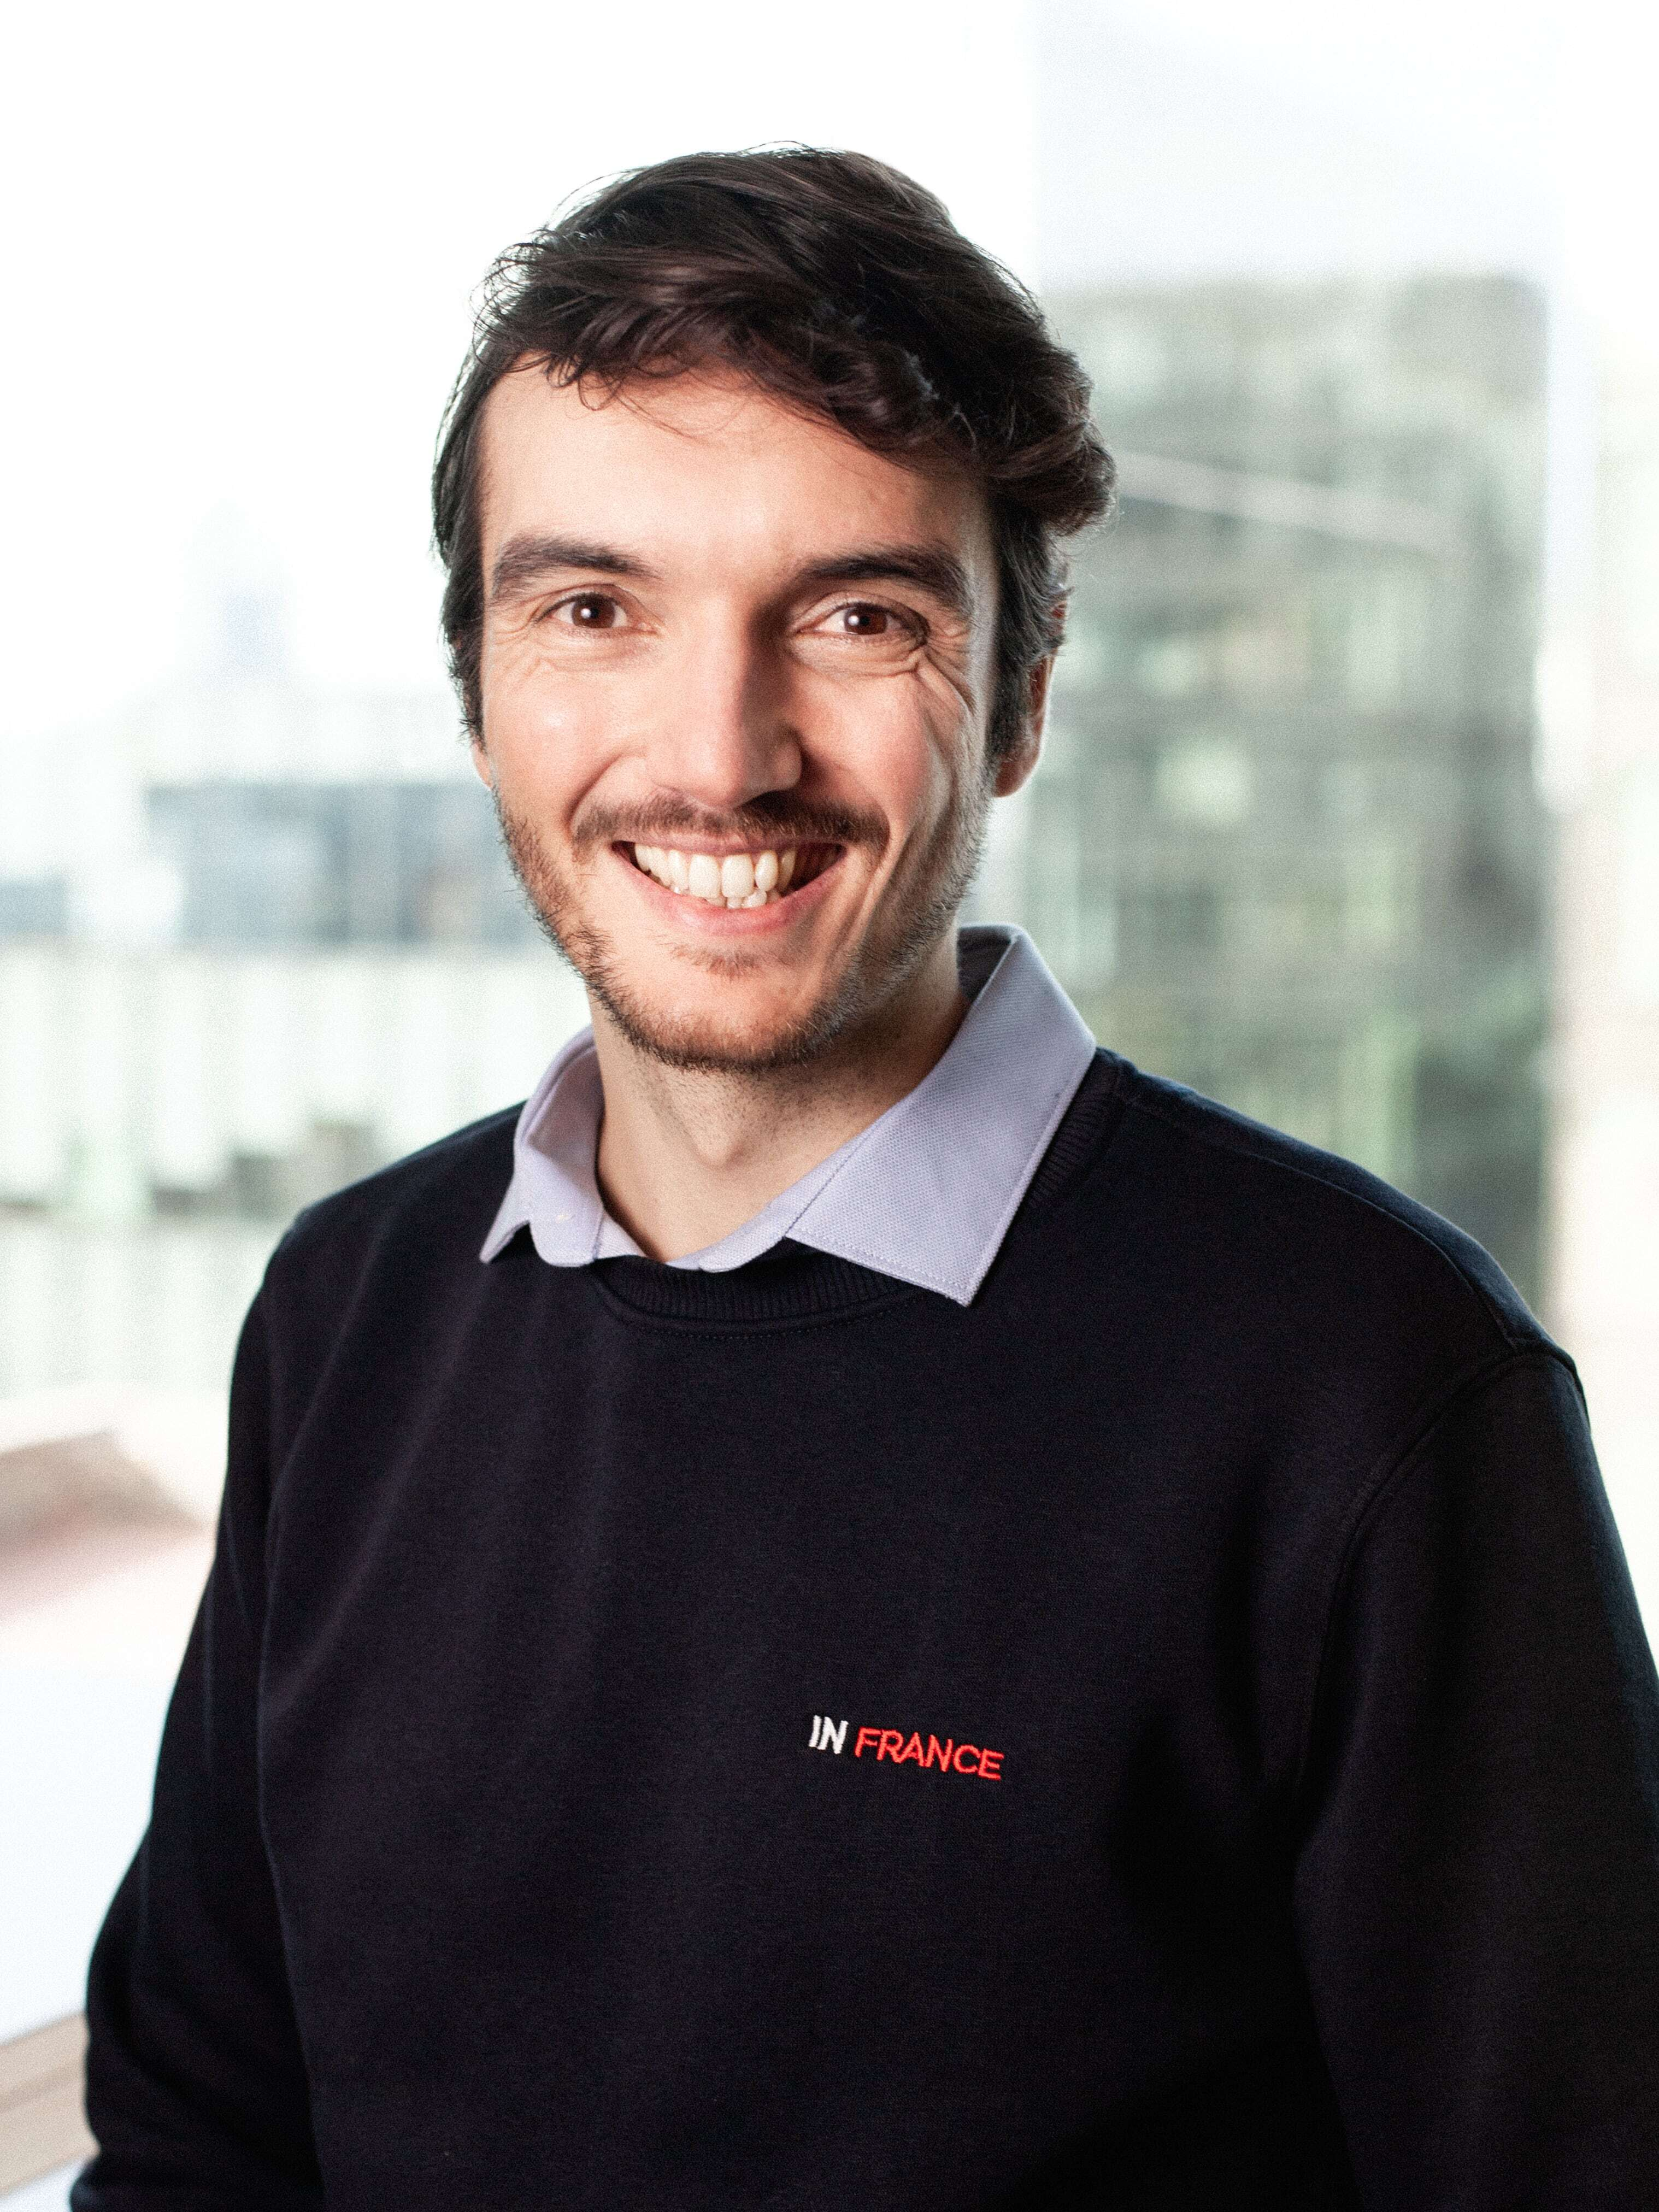
\includegraphics[width=5cm]{image/trombine-christophe}
        \end{columns}
    \end{frame}

\end{document}
